%iffalse
\let\negmedspace\undefined
\let\negthickspace\undefined
\documentclass[journal,12pt,onecolumn]{exam}
\usepackage[version=4]{mhchem}
\usepackage{chemformula} % for \ch if needed
\usepackage{chemfig}
\usepackage{chemmacros}
\chemsetup{modules = reactions} % Enables reaction arrows
\usepackage{graphicx}
\graphicspath{ {./images/} }

\usepackage{fancyhdr}
\usepackage{geometry}
\usepackage{lastpage}
\usepackage{cite}
\usepackage{amsmath,amssymb,amsfonts,amsthm}
\usepackage{enumitem,multicol}
\usepackage{algorithmic}
\usepackage{graphicx}
\usepackage{textcomp}
\usepackage{xcolor}
\usepackage{txfonts}
\usepackage{listings}
\usepackage{enumitem}
\usepackage{mathtools}
\usepackage{gensymb}
\usepackage{comment}
\usepackage[breaklinks=true]{hyperref}
\usepackage{tkz-euclide} 
\usepackage{listings}
\usepackage{gvv}                                        
%\def\inputGnumericTable{}                                 
\usepackage[latin1]{inputenc}                                
\usepackage{color}                                            
\usepackage{array}                                            
\usepackage{longtable}                                       
\usepackage{calc}                                             
\usepackage{multirow}                                         
\usepackage{hhline}                                           
\usepackage{ifthen}                                           
\usepackage{lscape}
\usepackage{tabularx}
\usepackage{array}
\usepackage{float}


\newtheorem{theorem}{Theorem}[section]
\newtheorem{problem}{Problem}
\newtheorem{proposition}{Proposition}[section]
\newtheorem{lemma}{Lemma}[section]
\newtheorem{corollary}[theorem]{Corollary}
\newtheorem{example}{Example}[section]
\newtheorem{definition}[problem]{Definition}
\newcommand{\BEQA}{\begin{eqnarray}}
\newcommand{\EEQA}{\end{eqnarray}}
\newcommand{\define}{\stackrel{\triangle}{=}}
\theoremstyle{remark}

\geometry{margin=1 in}

\pagestyle{fancy}
\fancyhead[L]{2011}
\fancyhead[C]{CY}
\fancyhead[R]{CY}
\fancyfoot[L]{CY}
\fancyfoot[C]{CY}
\fancyfoot[R]{Page \thepage}

\setlength{\headheight}{14pt}
\setlength{\headsep}{5pt}
\setlength{\footskip}{20pt}


% Line thickness
\renewcommand{\headrulewidth}{0pt}
\renewcommand{\footrulewidth}{0pt}



\pagestyle{fancy}
\fancyhf{} % clear all header and footer fields

\setlength{\headheight}{50pt} % Increase header height to fit image

\fancyhead[C]{%
  
\includegraphics[width=\textwidth]{figs/header.png}
}



\usepackage{fancyhdr}
\usepackage{graphicx}
\usepackage{geometry}
\geometry{a4paper, top=3.5cm}  % Adjust top margin to accommodate header

\usepackage{helvet}
\renewcommand{\familydefault}{\sfdefault}
\pagestyle{fancy}
\fancyfoot[C]{page \thepage}
\begin{document}
\textbf{\underline {GATE 2022 General Aptitude (GA)}}
\vspace{1em}

\begin{tabular}{|p{15cm}|}
\hline
\textbf{Q.1 -- Q.5 \ \ Carry ONE mark each.} \\
\hline
\end{tabular}
\vspace{1em}



\begin{enumerate}
    \item Inhaling the smoke from a burning \_\_\_\_\_\_\_\_ could \_\_\_\_\_\_\_\_ you quickly.
    \begin{enumerate}
        \item tire / tier
        \item tire / tyre
        \item tyre / tire
        \item tyre / tier
    \end{enumerate}



    \item A sphere of radius \( r \) cm is packed in a box of cubical shape.\\
    What should be the minimum volume (in cm\(^3\)) of the box that can enclose the sphere?
    
    \begin{enumerate}
        \item \( \frac{r^3}{8} \)
        \item \( r^3 \)
        \item \( 2r^3 \)
        \item \( 8r^3 \)
    \end{enumerate}

 \item Pipes P and Q can fill a storage tank in full with water in 10 and 6 minutes, respectively. Pipe R draws the water out from the storage tank at a rate of 34 litres per minute. P, Q and R operate at a constant rate.\\

    If it takes one hour to completely empty a full storage tank with all the pipes operating simultaneously, what is the capacity of the storage tank (in litres)?

    \begin{enumerate}
        \item 26.8
        \item 60.0
        \item 120.0
        \item 127.5
    \end{enumerate}
    \item Six persons P, Q, R, S, T and U are sitting around a circular table facing the center not necessarily in the same order. Consider the following statements:
    \begin{itemize}
        \item P sits next to S and T.
        \item Q sits diametrically opposite to P.
        \item The shortest distance between S and R is equal to the shortest distance between T and U.
    \end{itemize}
    Based on the above statements, Q is a neighbor of

    \begin{enumerate}
        \item U and S
        \item R and T
        \item R and U
        \item P and S
    \end{enumerate}
    \item A building has several rooms and doors as shown in the top view of the building given below. The doors are closed initially.\\

    What is the minimum number of doors that need to be opened in order to go from the point P to the point Q?

    \begin{center}
        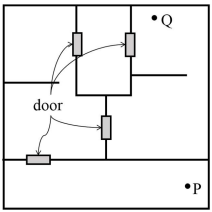
\includegraphics[width=0.4\textwidth]{figs/question number 4 .png} % Replace with actual image file
    \end{center}

    \begin{enumerate}
        \item 4
        \item 3
        \item 2
        \item 1
    \end{enumerate}
    \item Rice, a versatile and inexpensive source of carbohydrate, is a critical component of diet worldwide. Climate change, causing extreme weather, poses a threat to sustained availability of rice. Scientists are working on developing Green Super Rice (GSR), which is resilient under extreme weather conditions yet gives higher yields sustainably.\\

    Which one of the following is the CORRECT logical inference based on the information given in the above passage?

    \begin{enumerate}
        \item GSR is an alternative to regular rice, but it grows only in an extreme weather
        \item GSR may be used in future in response to adverse effects of climate change
        \item GSR grows in an extreme weather, but the quantity of produce is lesser than regular rice
        \item Regular rice will continue to provide good yields even in extreme weather
    \end{enumerate}
    
    \newpage
        \item A game consists of spinning an arrow around a stationary disk as shown below. When the arrow comes to rest, there are eight equally likely outcomes. It could come to rest in any one of the sectors numbered 1, 2, 3, 4, 5, 6, 7 or 8 as shown.\\

    Two such disks are used in a game where their arrows are independently spun.\\

    What is the probability that the sum of the numbers on the resulting sectors upon spinning the two disks is equal to 8 after the arrows come to rest?

    \begin{center}
        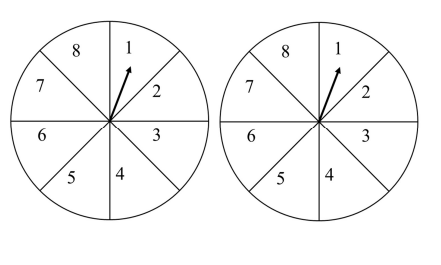
\includegraphics[width=0.5\textwidth]{figs/q 7.png} % Replace with the actual file name
    \end{center}

    \begin{enumerate}
        \item \( \frac{1}{16} \)
        \item \( \frac{5}{64} \)
        \item \( \frac{3}{32} \)
        \item \( \frac{7}{64} \)
    \end{enumerate}
    \vspace{2em}
     \item Consider the following inequalities.
    \begin{itemize}
        \item[(i)] \( 3p - q < 4 \)
        \item[(ii)] \( 3q - p < 12 \)
    \end{itemize}
    Which one of the following expressions below satisfies the above two inequalities?

    \begin{enumerate}[label=(\Alph*)]
        \item \( p + q < 8 \)
        \item \( p + q = 8 \)
        \item \( 8 \leq p + q < 16 \)
        \item \( p + q \geq 16 \)
    \end{enumerate}
    \newpage
     \item Given below are three statements and four conclusions drawn based on the statements.

    Statement 1: Some engineers are writers.\\
    Statement 2: No writer is an actor.\\
    Statement 3: All actors are engineers.\\

    \vspace{0.3em}
    Conclusion I: Some writers are engineers.\\
    Conclusion II: All engineers are actors.\\
    Conclusion III: No actor is a writer.\\
    Conclusion IV: Some actors are writers.\\

    Which one of the following options can be logically inferred?

    \begin{enumerate}
        \item Only conclusion I is correct
        \item Only conclusion II and conclusion III are correct
        \item Only conclusion I and conclusion III are correct
        \item Either conclusion III or conclusion IV is correct
    \end{enumerate}
    \item Which one of the following sets of pieces can be assembled to form a square with a single round hole near the center? Pieces cannot overlap.

    \begin{enumerate}
        \item 
        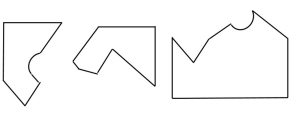
\includegraphics[width=0.4\textwidth]{figs/q10a.png}
        
        \item 
        
\includegraphics[width=0.4\textwidth]{figs/q10b.png}
        
        \item 
        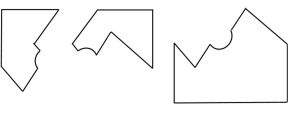
\includegraphics[width=0.4\textwidth]{figs/q10c.png}
        
        \item 
        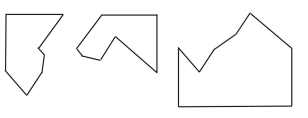
\includegraphics[width=0.4\textwidth]{figs/q10d.png}
    \end{enumerate}
\newpage
\textbf{GATE 2022 Humanities and Social Sciences - Economics (XH-C1)}\

\textbf{XH-B1: Q.11 - Q.17 Carry ONE mark Each }
 \item A relationship is expressed as Iodine : Goitre.\\
    The pair(s) of words showing SIMILAR relationship is/are

    \begin{enumerate}
        \item Mango : Anaemia
        \item Insulin : Diabetes
        \item Fat : Obesity
        \item Hormones : Heredity
    \end{enumerate}

    \item Three individuals are named P, Q, and R. Together they have a total of fifteen children of which nine are boys. P has three girls and Q has same number of boys. Q has one more child than P, who has four children. R has four more boys than the number of girls. The number of girls of R is equal to the number of boys of P. How many boys do R and P have?

    \begin{enumerate}
        \item R = 3, P = 3
        \item R = 4, P = 2
        \item R = 5, P = 1
        \item R = 2, P = 4
    \end{enumerate}
    \textbf{GATE 2022 Humanities and Social Sciences - Economics (XH-C1)}
 \item A sentence has been given below.\\

    \textit{The train will leave at 8:30 PM, we have been ready by 7:30 PM, so that we can reach the station on time.}\\

    To make the above sentence grammatically correct, the phrase marked in italics is to be replaced by

    \begin{enumerate}
        \item were
        \item are
        \item must be
        \item should have
    \end{enumerate}
    \newpage
    \item Complete the sentence correctly using the options given below.\\

    Hastings \_\_\_\_ $(p)$ \_\_\_\_ developed as a holiday resort after \_\_\_\_ $(q)$ \_\_\_\_.\\

    \begin{enumerate}
        \item $(p) =$ a seaside town, \quad $(q) =$ the first world war
        \item $(p) =$ a seaside town, \quad $(q) =$ the First World War
        \item $(p) =$ a Seaside Town, \quad $(q) =$ World War I
        \item $(p) =$ A seaside town, \quad $(q) =$ World War I
    \end{enumerate}
\textbf{GATE 2022 Humanities and Social Sciences - Economics (XH-C1)}
\item The Arecibo telescope does not resemble what most of us think of when we hear
the word telescope. Its reflective surface covers an area of 20 acres, which is quite
remarkable. Dangling above it are towers and cables, sub-reflectors and antennas,
all of which can be positioned using 26 motors to transmit radio waves and receive
echoes with astonishing precision.

\vspace{1em}

From the passage, it can be inferred that most telescopes 


\begin{enumerate}
    \item are not as large as Arecibo 
    \item not have reflective surface 
    \item cannot be re-positioned 
    \item strictly have 26 motors
\end{enumerate}
\textbf{GATE 2022 Humanities and Social Sciences - Economics (XH-C1)}
 \item Tailgating another vehicle is unsafe and illegal. Many rear-end collisions are caused by drivers following too close to the vehicle in front of them. The rules state that a driver must keep significant distance from the vehicle in front in order to stop safely and avoid a collision. Drivers should allow a minimum two seconds gap between their vehicle and the one ahead. At 60 km per hour, this equates to a gap of 33 meters; at 100 km per hour, it equates to a gap of 55 meters. More distance is needed to safely stop in rain or poor visibility, as during rain slippery roads reduce the effectiveness of braking.\\

    Which of the following statement(s) \textbf{can be inferred} from the above passage?

  
    

    \begin{enumerate}
        \item People drive faster in rain and under poor visibility.
        \item Braking may not be as effective during rain as in the dry conditions.
        \item Tailgating is against the road rules.
        \item Collision has no relationship with tailgating.
    \end{enumerate}


\item There are three separate, but equal-sized boxes. Inside each box, there are two
separate small boxes. Inside each of the small boxes, there are four even smaller
boxes. The total number of boxes will be\underline{\hspace{2cm}}.\\


\textbf{GATE 2022 Humanities and Social Sciences - Economics (XH-C1)}\ 

\textbf{Q.18 - Q.26 Carry TWO marks Each}
\item In a specific language, \textit{xer dan} means ``big horse'', \textit{liro cas} means ``red tomato'' and \textit{dum cas dan} means ``big red barn''. \\

  The equivalent word for \textbf{barn} in this language is \
  
  \begin{enumerate}
    \item \textit{dum}
    \item \textit{liro}
    \item \textit{dan}
    \item \textit{cas}
  \end{enumerate}
  
  \item Park street is parallel to Rock street. Garden street is perpendicular (90\degree) to Lake street. Lake street is parallel to Rock street. \\
  
  For the situation described above, the \textbf{TRUE statement} is \

  \begin{enumerate}
    \item Park street is perpendicular to Lake street
    \item Rock street is parallel to Garden street
    \item Park street is parallel to Garden street
    \item Garden street is perpendicular to Park street
  \end{enumerate}
\textbf{GATE 2022 Humanities and Social Sciences - Economics (XH-C1)}
 \item Six examinations are required to be conducted in a week starting from Sunday to Saturday. Hindi is not scheduled on the first day and English is not scheduled before Hindi. Mathematics is scheduled one day after Physics. Biology is scheduled two days after Hindi. One day prior to Chemistry, there is no examination. Only one examination can be scheduled on a single day and Sunday is not an off day. What are the subjects scheduled on first and the last days? \\
  
 
  \begin{enumerate}
    \item First day Physics, Last day Biology
    \item First day Physics, Last day Chemistry
    \item First day Physics, Last day English
    \item First day English, Last day Biology
  \end{enumerate}
  \newpage
  \textbf{GATE 2022 Humanities and Social Sciences - Economics (XH-C1)}
   \item A passage consists of 6 sentences. The first and sixth sentences of the passage are at their correct positions, while the middle four sentences (represented by P, Q, R, and S) are jumbled up.

\textit{First sentence:} Smoke oozed up between the planks.

\textbf{P:} Passengers were told to be ready to quit the ship.\\
\textbf{Q:} The rising gale fanned the smouldering fire.\\
\textbf{R:} Everyone now knew there was fire onboard.\\
\textbf{S:} Flames broke out here and there.

\textit{Sixth sentence:} Most people bore the shock bravely.

The \textbf{most logically CORRECT order} for the given jumbled up sentences is

\vspace{0.2cm}
Space for Figure/Equation, if any:
\begin{enumerate}
  \item \textbf{QSRP}
  \item \textbf{QPSR}
  \item \textbf{RSPQ}
  \item \textbf{PQRS}
\end{enumerate}
\textbf{GATE 2022 Humanities and Social Sciences - Economics (XH-C1)}
 \item For a painting to succeed, it is essential that the painter and his public agree about what is significant. The subject of the painting may have a personal meaning for the painter or a common person; but there can also be the possibility of their agreement on its general meaning. It is at this point that the culture of the society and the period in question precedes the artists and her/his art. Renaissance art would have meant nothing to the Aztecs, and vice versa. If, to some extent, a few intellectuals can appreciate them both today, it is because their culture is a historical one. Its inspiration is history and all known developments to date.

According to the passage, which of the following is/are \textbf{NOT necessarily} among the attributes needed for a painter to succeed?

\vspace{0.2cm}

\begin{enumerate}
  \item The subject must have a personal meaning for the painter.
  \item The painter is able to communicate and justify the significance of its subject selection.
  \item The painter and the public agree on what is significant.
  \item The painting of the subjects is driven by public demand.
\end{enumerate}

\newpage
\textbf{GATE 2022 Humanities and Social Sciences - Economics (XH-C1)}
\item Vinod has a pre-determined route. Each morning he delivers 37 newspapers to
customers in his neighborhood. It takes Vinod 50 minutes to deliver all the papers.
When Vinod was sick or had other engagements, his friend Tarun, who lives on the
same street delivered the papers on his behalf. 
\vspace{1em}
Find the statement(s) that must be \textbf{TRUE} according to the given information. 
\begin{enumerate}
    \item Vinod and Tarun lived in the same locality   
    \item It was dark outside when Vinod began his delivery. 
    \item It took Tarun more than 50 minutes to deliver the papers. 
    \item Tarun delivered 37 newspapers to customers. 
    
\end{enumerate}

\item Cholera, typhoid, diphtheria and tuberculosis cause huge number of deaths.Poor quality drinking water has always been the world's greatest single carrier of sickness. Disease is transmitted when sewage and drinking water come into contact.Children are particularly vulnerable. In some of the poorest countries the infant mortality rate is high. The separation of sewage and the supply of clean drinking water are the domain of civil engineers, and their work makes a significant contribution to public health. That contribution was recognized when public sanitation was voted the greatest medical breakthrough, beating the discoveries including antibiotics and vaccines in a poll organized by the British Medical Journal.

\vspace{1em}
Identify the statement(s), which is/are \textbf{NOT TRUE} according to the passage.
\begin{enumerate}
    \item Children are less prone to water borne diseases. 
    \item The infant mortality rate was high in economically weaker countries.
    \item The provision of sewage and drinking water should be adequately separated from each other. 
    \item The literature states that the public health and sanitation was never given its due importance. 

    
\end{enumerate}
\newpage

 \item Shark's teeth have evolved to correspond to the diet of each particular species of shark. Consequently, the teeth of the great white shark bear little resemblance to those of the bull shark or nurse shark. There were essentially four different shark diets and thus four varieties of shark teeth. Sharks that feed on fish have needle like teeth, perfect for spearing and ripping. Sharks that eat mammals such as seals and sea lions have heavy, serrated teeth, typically triangular on the upper jaw and pointed on the lower jaw. Shark that feed in the benthic zone of the ocean have flattened teeth for crushing the shell of the creatures they find scuttling in the sand or clinging to rocks. Sharks that bask have teeth that are largely non-functional; these sharks filter food from the water by passing it through their gills.

Which of the following is/are the \textbf{CORRECT inference(s)} as per the passage?

\vspace{0.2cm}
Space for Figure/Equation, if any:
\begin{enumerate}
  \item Shark's teeth are not specially designed for slaughter.
  \item The shape of the shark's teeth relates to its prey.
  \item Some species of sharks filter food through their gills.
  \item Shark's teeth relate to its diet.
\end{enumerate}
\item A particular school management wants to contact all parents, all businessmen and all engineers. The following statistics are available with the school.

\begin{itemize}
  \item Businessmen = 50
  \item Engineers = 25
  \item Parents = 2500
  \item Businessmen who are engineers = 0
  \item Businessmen who are parents = 25
  \item Engineers who are parents = 15
\end{itemize}

The number of people needs to be contacted are \underline{\hspace{2cm}}.

\newpage
\textbf{GATE 2022 Humanities and Social Sciences - Economics (XH-C1)}

\vspace{2em}

\textbf{XH-C1 (Q.27 - Q.35 Carry ONE mark Each)}
\item Suppose that a firm has a technology represented by the following production function:
  \[
    Y(K, L) = K^x L^y
  \]
  where $K$ denotes capital, $L$ denotes labour, $Y$ denotes the maximum output that is possible to produce using capital $K$ and labour $L$. $x$ and $y$ are two positive real numbers. It is also known that the production function satisfies constant returns to scale. Then which of the following is true?

  \begin{enumerate}
    \item $x + y = 0.5$
    \item $x + y = 1$
    \item $x + y = 1.5$
    \item $x + y = 2$
  \end{enumerate}
  
  \vspace{2em}

  \item The Human Development Index (HDI), as reported by the United Nations Development Program, is based on three components. Two of these components are per-capita income and a measure of educational attainment of society. The third component is

  \begin{enumerate}
    \item Gini coefficient
    \item percentage of population who have access to safe drinking water
    \item percentage of population who work in non-agricultural sector
    \item life expectancy at birth
  \end{enumerate}

 \item Suppose we estimate the following regression equation:
  \[
    \ln(x_t) = \alpha_0 + \alpha_1 \ln(y_t) + \varepsilon_t, \quad \alpha_0, \alpha_1 > 0
  \]
  where $x_t$ and $y_t$ are some variables. $\alpha_0$ and $\alpha_1$ are the intercept and the slope, respectively. $\varepsilon_t$ is the residual term. What is the interpretation of the coefficient $\alpha_1$?

  \begin{enumerate}
    \item A 1\% increase in $y_t$ causes a $\alpha_1$\% increase in $x_t$
    \item A 1\% increase in $y_t$ causes a $\alpha_1 \times 0.01$ unit increase in $x_t$
    \item A one unit increase in $y_t$ causes a $100 \times \alpha_1$\% increase in $x_t$
    \item A one unit increase in $y_t$ causes a $\alpha_1$ unit increase in $x_t$
  \end{enumerate}
  \newpage
   \item Consider the following system of equations in three variables $x, y, z$:
  \[
  \begin{aligned}
    -x - y - z &= 3 \\
    x + y + z &= 10 \\
    2x - 3y &= 6
  \end{aligned}
  \]
  This system of equations has

  \begin{enumerate}
    \item no combination of values of $(x, y, z)$ that satisfy this system simultaneously
    \item only one combination of values of $(x, y, z)$ that satisfy this system simultaneously
    \item only two combinations of values of $(x, y, z)$ that satisfy this system simultaneously
    \item infinitely many combinations of values of $(x, y, z)$ that satisfy this system simultaneously
  \end{enumerate}
  \item Which of the following models appropriately explains the fluctuations in potential output and long-run aggregate supply by understanding the shocks to productivity or the willingness of the worker?

  \begin{enumerate}[label=(\Alph*)]
    \item Solow growth model
    \item Real business cycle model
    \item IS-LM model
    \item Harrod-Domar Model
  \end{enumerate}

  \item The change in equilibrium output for an equal amount of change in government expenditure and tax revenue is linked to which one of the following multipliers?

  \begin{enumerate}
    \item Expenditure multiplier
    \item Balanced Budget multiplier
    \item Lum-sum tax multiplier
    \item Trade multiplier
  \end{enumerate}
  \newpage
\item Solaris is a firm that can install solar panels at an airport to generate electricity for the airport's usage. The company claims that in 70 percent of all airports where its solar panels are installed, an airport's electricity bill is reduced by at least 40 percent. The probability that an airport's electricity bill is reduced by at least 40 percent, in seven out of ten airports where the company's solar panels are installed, equals approximately:

  \begin{enumerate}
    \item 0.082
    \item 0.002
    \item 0.490
    \item 0.267
  \end{enumerate}

  \item IndiaSmart is a retail shop that accepts either a Rupay credit card, or a Visa credit card. 31 percent of IndiaSmart's customers carry a Rupay credit card, 44 percent of its customers carry a Visa credit card, while 18 percent of its customers carry a Rupay credit card as well as a Visa credit card. What is the probability that a customer carries at least one of the two, i.e. either a Rupay or a Visa credit card?

  \begin{enumerate}
    \item 0.75
    \item 0.93
    \item 0.57
    \item 0.49
  \end{enumerate}

   \item What is the user cost of capital for a firm when the rate of depreciation of machine is 20\% and the cost of financial capital is 15\%?

  \begin{enumerate}
    \item 37\%
    \item 50\%
    \item 35\%
    \item 31\%
  \end{enumerate}

  \item Which among the following Gini coefficients exhibits the highest equality?

  \begin{enumerate}
    \item 0.1
    \item 0.2
    \item 0.5
    \item 0.6
  \end{enumerate}

\newpage
 \item Let $f(x,y)$ be a continuously differentiable homogeneous function of degree 4. Which of the following is necessarily true?

  \begin{enumerate}
    \item $x \dfrac{\partial f(x,y)}{\partial x} + y \dfrac{\partial f(x,y)}{\partial y} = f(x,y)$
    \item $x \dfrac{\partial f(x,y)}{\partial x} + y \dfrac{\partial f(x,y)}{\partial y} = 2f(x,y)$
    \item $x \dfrac{\partial f(x,y)}{\partial x} + y \dfrac{\partial f(x,y)}{\partial y} = 4f(x,y)$
    \item $\dfrac{\partial f(x,y)}{\partial x} + \dfrac{\partial f(x,y)}{\partial y} = 8f(x,y)$
  \end{enumerate}

  \item Which of the following committees was set-up to address issues related to capital account convertibility in India?

  \begin{enumerate}
    \item Tandon Committee
    \item Abid Hussain Committee
    \item Tarapore Committee
    \item Percy Mistry Committee
  \end{enumerate}
  \item The demand curve for tea in Borduria is given by
  \[
  D(P) = 40 - 2P
  \]
  and the domestic supply curve of tea in Borduria is given by
  \[
  S(P) = \frac{2}{3}P
  \]
  Here $D(P)$ denotes quantity demanded when price is $P$ and $S(P)$ is quantity supplied by domestic producers at price $P$. Tea is traded in a competitive world market and imported into Borduria at a price of 9 per unit. Initially there was no restriction on trade. However, as a result of lobbying by the domestic suppliers, the Bordurian government imposes a tariff of 3 per unit on each unit imported. 

  As a result of the tariff, import of tea decreased by how many units?

  \begin{enumerate}
    \item 2
    \item 3
    \item 8
    \item 9
  \end{enumerate}
\newpage
\item Bretton Woods agreement gave birth to the following organization: 
\begin{enumerate}
    \item GATT
    \item RBI
    \item NAFTA
    \item ASEAN
\end{enumerate}
\item Which one of the following is a test of heteroscedasticity?
  \begin{enumerate}
    \item White test
    \item Jarque-Bera test
    \item Breusch-Godfrey test
    \item Ljung-box test
  \end{enumerate}

  \item The law that explains the relationship between income growth and the size of government expenditure is appropriately linked to:
  \begin{enumerate}
    \item Wagner's law
    \item Okun's law
    \item Walras law
    \item Ricardian equivalence
  \end{enumerate}

  \item As per recent Economic Survey, how many states and Union Territories (UTs) are driven by services sector in India?
  \begin{enumerate}
    \item 15
    \item 19
    \item 25
    \item 21
  \end{enumerate}

\item An economy is characterized by the following production function:
  \[
  Y = A K^{0.25} L^{0.75}
  \]
  where \(K\) denotes capital, \(L\) denotes labour, \(A\) denotes the total factor productivity and \(Y\) denotes output produced. All capital and labour are fully employed. Suppose that the growth rate of labour is 1%, the growth rate of capital is 4%, and the growth rate of output is 4%. The growth rate of total factor productivity \(A\) is
  \begin{enumerate}
    \item 1.5\%
    \item 1.75\%
    \item 2.25\%
    \item 2.5\%
  \end{enumerate}

\newpage
\textbf{Q.45 - Q.65 Carry TWO marks Each}

\item Suppose a firm has the following production function:
  \[
  f(x_1, x_2, x_3, x_4) = \min\{x_1, x_2\} + \min\{x_3, x_4\}
  \]
  The per unit cost of input \(x_i\) is given by \(w_i\), where \(i = 1, 2, 3, 4\). Suppose that \(w_1 = 1\), \(w_2 = 5\), \(w_3 = 3\), and \(w_4 = 6\). If the firm is minimizing cost, which of the following input choices by the firm can be observed?
  \begin{enumerate}
    \item \(x_1 > 0, x_2 = 0, x_3 > 0, x_4 = 0\)
    \item \(x_1 > 0, x_2 = 0, x_3 = 0, x_4 = 0\)
    \item \(x_1 > 0, x_2 = 0, x_3 = 0, x_4 > 0\)
    \item \(x_1 = 0, x_2 = 0, x_3 > 0, x_4 > 0\)
  \end{enumerate}

  \item Suppose an econometrician had specified the following regression:
  \[
  y_t = \beta_1 + \beta_2 z_{2t} + \beta_3 z_{3t} + \beta_4 z_{4t} + \varepsilon_t
  \]
  but a researcher estimated the following regression:
  \[
  y_t = \beta_1 + \beta_2 z_{2t} + \beta_3 z_{3t} + \beta_4 z_{4t} + \beta_5 z_{5t} + \varepsilon_t
  \]
  What will be the consequence of including the irrelevant variable on the estimated coefficients?
  \begin{enumerate}
    \item Coefficient estimates will be unbiased, consistent but inefficient
    \item Coefficient estimates will be consistent, asymptotically efficient but biased
    \item Coefficient estimates will be inconsistent and efficient
    \item Coefficient estimates will be biased, consistent and efficient
  \end{enumerate}
\newpage
\item Okun's law says that a 1% increase in unemployment for one year is associated with a 2% decrease in GDP growth. Suppose an economy has the following expectations augmented Phillips curve:
  \[
  \pi = \pi^e - \beta(U - U^N), \quad \beta > 0
  \]
  where \(\pi\) and \(\pi^e\) are the inflation and expected inflation rates, respectively. \(U\) and \(U^N\) are the unemployment and natural rate of unemployment, respectively. \(\beta\) measures sensitivity of inflation to unemployment gap. When \(\beta = 2\), by what percentage does output fall short of full-employment given that the inflation rate, expected inflation rate and natural rate of unemployment are 8%, 10% and 6%, respectively?
  \begin{enumerate}
    \item 2
    \item 4
    \item 6
    \item 8
  \end{enumerate}

  \item Let \(f(x)\) be the probability distribution function of a random variable \(X\), where
  \[
  f(x) = \frac{5x^4}{64} \quad \text{if } -2 < x < 2
  \]
  \[
  = 0 \quad \text{otherwise}
  \]
  Let \(|\cdot|\) denote the modulus function. Then, \(\mathrm{P}(|X| < 1)\) and \(\mathrm{P}(X^2 < 3)\) are given by (respectively):
  \begin{enumerate}
    \item \((1/32)\) and \(9(\sqrt{3}/32)\)
    \item \((5/64)\) and \(5(\sqrt{3}/32)\)
    \item \((1/64)\) and \((\sqrt{3}/32)\)
    \item \(2(\sqrt{3}/32)\) and \((1/32)\)
  \end{enumerate}
\item Liquidity Adjustment Facility (LAF) uses the following instruments:
  \begin{enumerate}
    \item Call Money Rate and Mumbai Inter-bank Offered Rate
    \item Repo Rate and Reverse Repo Rate
    \item Bank Rate and Statutory Liquidity Ratio
    \item Cash Reserve Ratio and Prime Lending Rate
  \end{enumerate}

  \item What is the weightage of manufacturing sector in the Index of Industrial Production (IIP) during 2020-2021? \\
  \textit{Note: numbers are in approximate values}
  \begin{enumerate}
    \item 78\%
    \item 81\%
    \item 65\%
    \item 71\%
\end{enumerate}

 \item The curve that explains the relationship between tax rate and tax revenue is known as:
  \begin{enumerate}
    \item Laffer curve
    \item Engle curve
    \item Beveridge curve
    \item Phillips curve
  \end{enumerate}

  \item Suppose the estimated consumption equation of an economy is:
  \[
    C = 40 + \beta Y_d
  \]
  where $Y_d$ is the personal disposable income, $\beta$ is the marginal propensity to consume (MPC). Government expenditure ($G$) is given as 90. Total tax ($T$) received is $\delta Y$, where $Y$ is aggregate output or real income and $\delta$ is tax to real income proportionality factor. Autonomous investment ($I_a$) is given as 80. What are the tax revenue and budget surplus of the government when $\beta = 0.75$ and $\delta = 0.20$? All units are measured in constant rupees.

  \begin{enumerate}
    \item Tax revenue = Rs. 105 and surplus = Rs. 15
    \item Tax revenue = Rs. 118 and surplus = Rs. 28
    \item Tax revenue = Rs. 110 and surplus = Rs. 20
    \item Tax revenue = Rs. 125 and surplus = Rs. 35
  \end{enumerate}

\item Consider a two-period consumption model in which a representative household lives for two periods only. In period 1, he earns income $y_1$ and consumes $c_1$. In period 2, he earns $y_2$ and consumes $c_2$. He can borrow and lend at the same rate of interest ($r$). His lifetime utility function is as follows:

  \[
  U(c_1, c_2) = \ln(c_1) + \beta \ln(c_2)
  \]

  where $\beta > 0$ measures the sensitivity of future period's consumption. What will be the marginal propensity to consume of current consumption, i.e. $\frac{\partial c_1}{\partial y_1}$:

  \begin{enumerate}[label=(\Alph*)]
    \item $\frac{1}{1+\beta}$
    \item $\frac{1}{1+\beta^2}$
    \item $\frac{y_1}{1+\beta}$
    \item $\frac{y_1}{1+\beta^2}$
  \end{enumerate}
  \newpage

  \item Suppose an investigator has specified the following simultaneous equation model:
  \[
  y_{1t} = \alpha_{1,0} + \alpha_{1,2} y_{2t} + \alpha_{2} M_t + \alpha_3 K_t + u_t \quad (1)
  \]
  \[
  y_{2t} = \alpha_{2,0} + \alpha_{2,2} y_{1t} + \alpha_4 I_t + v_t \quad (2)
  \]

  where $y_{1t}$ and $y_{2t}$ are endogenous variables, $M_t$, $K_t$ and $I_t$ are predetermined variables. $u_t$ and $v_t$ are residual terms. Based on the order condition of identification, which one of the following statements are correct?

  \begin{enumerate}
    \item Equations (1) and (2) are exactly identified
    \item Equation (1) is exactly identified and equation (2) is over-identified
    \item Equation (1) is over-identified and equation (2) is exactly identified
    \item Both the equations are under-identified
  \end{enumerate}

\vspace{1em}

  \item There are two regions in a country. The demand for chocolates in region 1 is given by
  \[
  Q_1(P) = 100 - P
  \]
  and the demand for chocolates in region 2 is given by
  \[
  Q_2(P) = 200 - P
  \]
  where $Q_1(P)$ and $Q_2(P)$ denote the demand for chocolates in region 1 and 2 respectively at a price $P$. There is only one seller who is licensed to sell chocolates in the country. Suppose the seller sets a price of $P = 125$. The total demand for chocolates in the country at this price is

  \begin{enumerate}
    \item 50
    \item 75
    \item 100
    \item 125
  \end{enumerate}

 \newpage

 \item A producer manufactures batteries by using techniques I and II. The capacities (in ampere hours) of 12 randomly selected batteries manufactured by using technique I are: 140, 132, 136, 142, 138, 150, 154, 150, 152, 136, 144 and 142. Moreover, the capacities (in ampere hours) of 14 randomly selected batteries manufactured by using technique II are: 144, 134, 132, 130, 136, 146, 140, 128, 131, 128, 150, 137, 130 and 135.

  Suppose that battery capacities manufactured by using techniques I and II are normally distributed, with unknown means, $\mu_1$ and $\mu_{II}$ respectively, and an unknown common variance $\sigma^2$. Consider the null hypothesis $H_0$: $(\mu_1 - \mu_{II}) = \gamma$ ampere hours.

  For which of the following values of $\gamma$ should the null hypothesis $H_0$ be accepted, against the alternative hypothesis $H_1$: $(\mu_1 - \mu_{II}) \neq \gamma$ ampere hours, at 10\% level of significance?

  Note that if $Z$ is a standard normal variate, then: $P(Z \leq 1.282) = 0.900$, $P(Z \leq 1.645) = 0.950$, $P(Z \leq 1.960) = 0.975$ and $P(Z \leq 2.326) = 0.990$

  Further, if a random variable $T$ follows the Student's $t$-distribution, with degrees of freedom $r$, then the $\alpha$-percentile values $t_{\alpha,r}$ for various values of $\alpha$ and $r$ are given by (where $P(T \leq t_{\alpha,r}) = \alpha$):

  \[
  t_{0.90,24} = 1.318, \quad t_{0.90,25} = 1.316, \quad t_{0.90,26} = 1.315, \quad t_{0.95,24} = 1.711, \quad t_{0.95,25} = 1.708,\]
  \[\quad t_{0.95,26} = 1.706, \quad t_{0.975,24} = 2.064, \quad t_{0.975,25} = 2.060, \quad t_{0.975,26} = 2.056
  \]


  \begin{enumerate}
    \item $\gamma = 4$
    \item $\gamma = 7$
    \item $\gamma = 10$
    \item $\gamma = 13$
  \end{enumerate}

  \newpage

  \item Tom and Jerry both arrive at a petrol pump. Without worrying about price, Tom says, ``I want 10 liters of petrol.'' Also, without worrying about price, Jerry says, ``I want petrol worth 1000 rupees.'' The own price elasticities of demand for Tom (denoted by $\varepsilon_T$) and Jerry (denoted by $\varepsilon_J$) are:
  
  \begin{enumerate}
    \item $\varepsilon_T = 0, \quad \varepsilon_J = -\infty$
    \item $\varepsilon_T = 0, \quad \varepsilon_J = -1$
    \item $\varepsilon_T = -\infty, \quad \varepsilon_J = 0$
    \item $\varepsilon_T = -1, \quad \varepsilon_J = 0$
  \end{enumerate}

  \item Which of the following variables are pushed upwards by \textit{Seigniorage}?

  \begin{enumerate}
    \item Money supply
    \item Inflation
    \item Tax rate
    \item Interest rate
  \end{enumerate}

  \item Suppose Raju enters the job market at age 25 and earns annual income of Rs. 6000. He retires at age 65 and his life expectancy is 75 years. He does not own any assets. Assume that Raju consumes annual income uniformly over his lifetime. What will be his average propensity to consume during employment years?

  \begin{enumerate}
    \item 0.90
    \item 0.80
    \item 0.50
    \item 0.40
  \end{enumerate}

  \item A monopolist faces the following inverse demand function:
  \[
    P = 40 - Q,
  \]
  where \(P\) denotes price and \(Q\) denotes quantity. The monopolist has zero fixed cost and a marginal cost of 5 per unit of output produced. The monopolist aims to maximize profit. Suppose the government imposes a tax of 5 per unit of output on the monopolist. As a result, the price charged by the profit-maximizing monopolist to the consumer increases by:

  \begin{enumerate}
    \item 0
    \item 2.5
    \item 5
    \item 10
  \end{enumerate}
  \newpage

  \item In the flexible exchange rate environment with perfect capital mobility, a fiscal stimulus will be linked to which of the following statements?

  \begin{enumerate}[label=(\Alph*)]
    \item Fiscal policy increases the domestic outcome
    \item Fiscal policy does not increase the domestic output
    \item Fiscal policy leads domestic exports to fall
    \item Fiscal policy appreciates the domestic currency
  \end{enumerate}
\vspace{2em}
  \item Consider a lottery with two possible outcomes:
  \begin{itemize}
    \item Rupees 100 with probability 0.6
    \item Rupees 50 with probability 0.4
  \end{itemize}
  The maximum amount that a risk-neutral person would be willing to pay to play the above lottery equals Rupees \_\_\_\_\_\_ (in integer).

  \vspace{2em}

  \item Mr. Sharma's consumption preference for tea (denoted by \(x\)) and sugar (denoted by \(y\)) is given by the utility function
  \[
    U(x,y) = \min \{x, 2y\}
  \]
  The price per unit of tea is 10 and the price per unit of sugar is 10. Mr. Sharma's total income is 900.

  The optimum quantity of tea purchased by Mr. Sharma equals \_\_\_\_\_\_ (in integer).

  \item Suppose \(a\) is a real number between 0 and 1. Rohit is choosing \(x\) and \(y\) to maximize the following utility function:
  \[
  U(x,y) = x^2 + 2xy + y^2 + 4a^2 + 8a + 10
  \]
  subject to the following constraints:
  \[
  2x + y = 10, \quad x,y \geq 0
  \]
  Then the optimal value of \(y\) chosen by Rohit is \_\_\_\_\_\_ (in integer).

  \item In a competitive market for dry-cleaning, the inverse market demand function is given by
  \[
  P = 100 - Q
  \]
  where \(P\) denotes price and \(Q\) denotes quantity. The (private) marginal cost (MC) of production for all the dry-cleaning firms together is given by
  \[
  MC = 20 + 2Q
  \]
  The market pollution generated by the dry-cleaning processes of all firms creates external damages given by the marginal external cost (MEC):
  \[
  MEC = 20
  \]
  The socially efficient output of dry-cleaning is \_\_\_\_\_\_ (in integer).





  









\end{enumerate}
\end{document}
If you want me to compile all questions together or need any tweaks, just ask!



Ask ChatGPT

\end{document} 

